\documentclass[12pt]{article}
\usepackage[margin=1in]{geometry}
\usepackage[utf8]{inputenc}
\usepackage[english]{babel}
\usepackage[T1]{fontenc}
\usepackage{fourier}
\usepackage{amsthm}
\usepackage{amssymb}
\usepackage{amsmath}
\usepackage{amsfonts}
\usepackage{latexsym}
\usepackage{graphicx}
\usepackage{float}
\usepackage{etoolbox}
\usepackage{hyperref}
\usepackage{tikz}
\usepackage{lipsum}
\usepackage{algorithm}
\usepackage{algpseudocode}

\newcommand{\R}{\mathbb{R}}
\newcommand{\N}{\mathbb{N}}
\newcommand{\Z}{\mathbb{Z}}
\newcommand{\Q}{\mathbb{Q}}
\newcommand{\C}{\mathbb{C}}
\newcommand{\s}{\vspace*{0.4cm}}
\newcommand{\nd}{\noindent}

% add counters

\title{Spatial networks and small worlds}
\author{Luca Lombardo}
\date{December 2022}

\begin{document}
\maketitle

\begin{abstract}
    \noindent \lipsum[1]
\end{abstract}

\tableofcontents
\clearpage


\section{Introduction}

\subsection{Graph Theory}

\lipsum[1]


\subsection{Aim of the project}
Given a social network, which of its nodes are more central? This question has been asked many times in sociology, psychology and computer science, and a whole plethora of centrality measures (a.k.a. centrality indices, or rankings) were proposed to account for the importance of the nodes of a network. \s

\nd These networks, typically generated directly or indirectly by human activity and interaction (and therefore hereafter dubbed social”), appear in a large variety of contexts and often exhibit a surprisingly similar structure. One of the most important notions that researchers have been trying to capture in such networks is “node centrality”: ideally, every node (often representing an individual) has some degree of influence or importance within the social domain under  consideration, and one expects such importance to surface in the structure of the social network; centrality is a quantitative measure that aims at revealing the importance of a node. \s

\nd Among the types of centrality that have been considered in the literature, many have to do with distances between nodes. Take, for instance, a node in an undirected connected network: if the sum of distances to all other nodes is large, the node under consideration is peripheral; this is the starting point to define Bavelas's closeness centrality \cite{closeness}, which is the reciprocal of peripherality (i.e., the reciprocal of the sum of distances to all other nodes). \s

\nd The role played by shortest paths is justified by one of the most well-known features of complex networks, the so-called small-world phenomenon. A small-world network \cite{cohen_havlin_2010} is a graph where the average distance between nodes is logarithmic in the size of the network, whereas the clustering coefficient is larger (that is, neighborhoods tend to be denser) than in a random Erdős-Rényi graph with the same size and average distance. The fact that social networks (whether electronically mediated or not) exhibit the small-world property is known at least since Milgram's famous experiment \cite{} and is arguably the most popular of all features of complex networks. For instance, the average distance of the Facebook graph was recently established to be just $4.74$ \cite{milgram1967small}. \s

% \subsection*{Definitions and conventions}

% From now on, we consider directed graphs defined by a set $N$ of $n$ nodes and $A \subseteq N \times N$ of arcs. We write $x \to y$ when $(x,y) \in A$ and call $x$ and $y$ the source and the target of the arc, respectively. \s
% \clearpage




% \nd We are interest in analyzing 4 different centrality measures:

% \begin{itemize}
%     \item Distribution of Degree
%     \item Clustering coefficient
%     \item Average Path Length
%     \item Betweenness Centrality
% \end{itemize}
% \clearpage

\clearpage
% \section{Theoretical background on centrality measures}

% Centrality is a fundamental tool in the study of social networks: the first efforts to define formally centrality indices were put forth in the late 1940s by the Group Networks Laboratory at MIT directed by Alex Bavelas \cite{closeness}; those pioneering experiments concluded that centrality was related to group efficiency in problem-solving, and agreed with the subjects' perception of leadership. In the following decades, various measures of centrality were employed in a multitude of contexts. \s

% \subsection*{Geometric measures}

% We call geometric those measures assuming that importance is a function of distances; more precisely, a geometric centrality depends only on how many nodes exist at every distance. These are some of the oldest measures defined in the literature.

% \paragraph*{In-degree centrality} Indegree, the number of incoming arcs $d^-(x)$, can be considered a geometric measure: it is simply the number of nodes at distance one\footnote{Most centrality measures proposed in the literature were actually described only for undirected, connected graphs. Since the study of web graphs and online social networks has posed the problem of extending centrality concepts to networks that are directed, and possibly not strongly connected, in the rest of this paper we consider measures depending on the incoming arcs of a node (e.g., incoming paths, left dominant eigenvectors, distances from all nodes to a fixed node). If necessary, these measures can be called “negative”, as opposed to the “positive” versions obtained by considering outgoing paths, or (equivalently) by transposing the graph.} . It is probably the oldest measure of importance ever used, as it is equivalent to majority voting in elections (where $x \to y$ if $x$ voted for $y$). Indegree has a number of obvious shortcomings (e.g., it is easy to spam), but it is a good baseline. \s

% \nd Other notable geometric measures that we will not explore in this project, are \emph{closeness centrality}, (which is the reciprocal of the sum of distances to all other nodes, and betweenness centrality, which is the number of shortest paths that pass through a node), \emph{Lin's index} (which is the sum of the distances to all other nodes), and \emph{Harmonic Centrality} (which is a generalization of the closeness centrality). \s

% \clearpage

% \subsection*{Path-based measures}

% Path-based measures exploit not only the existence of shortest paths but actually take into examination all shortest paths (or all paths) coming into a node. We remark that in-degree can be considered a path-based measure, as it is the equivalent to the number of incoming paths of length one.

% \paragraph*{Betweenness centrality} Betweenness centrality  was introduced for edges, and then rephrased. The idea is to measure the probability that a random shortest path passes through a given node: if $\sigma_{yz}$ is the number of shortest paths going from $y$ to $z$, and $\sigma{yz}(x)$ is the number of such paths that pass through $x$, we define the betweenness of $x$ as

% \begin{equation}
%     \label{eq:betweenness}
%     \beta(x) = \sum_{y \neq x \neq z} \frac{\sigma_{yz}(x)}{\sigma_{yz}}.
% \end{equation}

% \nd The intuition behind betweenness is that if a large fraction of shortest paths passes through $x$, then $x$ is an important junction point of the network. Indeed, removing nodes in betweenness order causes a very quick disruption of the network.

\section{The Erdős-Rényi model}

\nd Before 1960, graph theory mainly dealt with the properties of specific individual graphs. In the 1960s, Paul Erdős and Alfred Rényi initiated a systematic study of random graphs. Random graph theory is, in fact, not the study of individual graphs, but the study of a statistical ensemble of graphs (or, as mathematicians prefer to call it, a \emph{probability space} of graphs). The ensemble is a class consisting of many different graphs, where each graph has a probability attached to it. A property studied is said to exist with probability $P$ if the total probability of a graph in the ensemble possessing that property is $P$ (or the total fraction of graphs in the ensemble that has this property is $P$). This approach allows the use of probability theory in conjunction with discrete mathematics for studying graph ensembles.  A property is said to exist for a class of graphs if the fraction of graphs in the ensemble which does not have this property is of zero measure. This is usually termed as a property of \emph{almost every (a.e.)} graph. Sometimes the terms “almost surely” or “with high probability” are also used (with the former usually taken to mean that the residual probability vanishes exponentially with the system size). \s


\subsection{Erdős-Rényi graphs}

\nd Two well-studied graph ensembles are $G_{N,M}$, the ensemble of all graphs with $N$ nodes and $M$ edges, and $G_{N,p}$, the ensemble of all graphs with $N$ nodes and probability $p$ of any two nodes being connected. These two families, initially studied by Erdős and Rényi, are known to be similar if $M = \binom{N}{2} p$, so as long $p$ is not too close to $0$ or $1$ they are referred to as ER graphs. \s

\nd An important attribute of a graph is the average degree, i.e., the average number of edges connected to each node. We will denote the degree of the ith node by $k_i$ and the average degree by $ \langle r \rangle $ . $N$-vertex graphs with $\langle k \rangle = O(N^0)$ are called sparse graphs. \s

\nd An interesting characteristic of the ensemble $G_{N,p}$ is that many of its properties have a related threshold function, $p_t(N)$, such that the property exists, in the “thermodynamic limit” of $N \to \infty$  with probability 0 if $p < p_t$ , and with probability $1$ if $p > p_t$ . This phenomenon is the same as the physical concept of a percolation phase transition. \s

\nd Another property is the average path length between any two nodes, which in almost every graph of the ensemble (with $\langle k \rangle > 1$ and finite) is of order $\ln N$ . The small, logarithmic distance is actually the origin of the “small-world” phenomena that characterize networks.


\subsection{Scale-free networks}

\nd The Erdős-Rényi model has traditionally been the dominant subject of study in the field of random graphs. Recently, however, several studies of real-world networks have found that the ER model fails to reproduce many of their observed properties. One of the simplest properties of a network that can be measured directly is the degree distribution, or the fraction P(k) of nodes having k connections (degree $k$). A well-known result for ER networks is that the degree distribution is Poissonian,

\begin{equation}
    P(k) = \frac{e^{z} z^k}{k!}
\end{equation}

\nd Where $z = \langle k \rangle$. is the average degree. \s Direct measurements of the degree distribution for real networks show that the Poisson law does not apply. Rather, often these nets exhibit a scale-free degree distribution:

\begin{equation}
    P(k) = ck^{-\gamma} \quad \text{for} \quad k = m, ... , K
\end{equation}

\nd Where $c \sim (\gamma -1)m^{\gamma - 1}$ is a normalization factor, and $m$ and $K$ are the lower and upper cutoffs for the degree of a node, respectively. The divergence of moments higher then $\lceil \gamma -1 \rceil$ (as  $K \to \infty$ when $N \to \infty$) is responsible for many of the anomalous properties attributed to scale-free networks. \s

\nd All real-world networks are finite and therefore all their moments are finite. The actual value of the cutoff K plays an important role. It may be approximated by noting that the total probability of nodes with $k > K$ is of order $1/N$

\begin{equation}
    \int_K^\infty P(k) dk \sim \frac{1}{N}
\end{equation}

\nd This yields the result

\begin{equation}
    K \sim m N^{1/(\gamma -1)}
\end{equation}

\nd The degree distribution alone is not enough to characterize the network. There are many other quantities, such as the degree-degree correlation (between connected nodes), the spatial correlations, the clustering coefficient, the betweenness or central-ity distribution, and the self-similarity exponents.

\subsection{Diameter and fractal dimension}

Regular lattices can be viewed as networks embedded in Euclidean space, of a well-defined dimension, $d$. This means that $n(r)$, the number of nodes within a distance $r$ from an origin, grows as $n(r) \sim r^d$ (for large $r$). For fractal objects, $d$ in the last relation may be a non-integer and is replaced by the fractal dimension $d_f$ \s

\nd An example of a network where the above power laws are not valid is the Cayley tree (also known as the Bethe lattice). The Cayley tree is a regular graph, of fixed degree $z$, and no loops. An infinite Cayley tree cannot be embedded in a Euclidean space of finite dimensionality. The number of nodes at $l$ is $n(l) \sim (z - 1)^l$ . Since the exponential growth is faster than any power law, Cayley trees are referred to as infinite-dimensional systems. \s

\nd In most random network models, the structure is locally tree-like (since most loops occur only for $n(l) \sim N$), and since the number of nodes grows as $n(l) \sim \langle k - 1 \rangle^l$, they are also infinite dimensional. As a consequence, the diameter of such graphs (i.e., the minimal path between the most distant nodes) scales as $D \sim \ln N$. Many properties of ER networks, including the logarithmic diameter, are also present in Cayley trees. This small diameter in ER graphs and Cayley trees is in contrast to that of finite-dimensional lattices, where $D \sim N^{1/d_l}$. \s

\nd Similar to ER, percolation on infinite-dimensional lattices and the Cayley tree  yields a critical threshold $p_c = 1/(z - 1)$. For $p > p_c$, a “giant cluster” of order $N$ exists, whereas for $p < pc$,only small clusters appear. For infinite-dimensional lattices (similar to ER networks) at criticality, $p =
p_c$ , the giant component is of size $N^{2/3}$. This last result follows from the fact that percolation on lattices in dimension $d \geq d_c = 6$ is in the same universality class as infinite-dimensional percolation, where the fractal dimension of the giant cluster is $d_f = 4$, and therefore the size of the giant cluster scales as $N^{d_f/d_c} = N^{2/3}$. The dimension $d_c$ is called the “upper critical dimension.” Such an upper critical dimension exists not only in percolation phenomena, but also in other physical models, such as in the self-avoiding walk model for polymers and in the Ising model for magnetism; in both these cases $d_c = 4$.

\nd Watts and Strogatz suggested a model that retains the local high clustering of lattices (i.e., the neighbors of a node have a much higher probability of being neighbors than in random graphs) while reducing the diameter to $D \sim \ln N$ . This so-called, “small-world network” is achieved by replacing a fraction $\varphi$ of the links in a regular lattice with random links, to random distant neighbors. \s

\subsection{Random graphs as a model of real networks}

\nd Many natural and man-made systems are networks, i.e., they consist of objects and interactions between them. These include computer networks, in particular the Internet, logical networks, such as links between WWW pages, and email networks, where a link represents the presence of a person's address in another person's address book. Social interactions in populations, work relations, etc. can also be modeled by a network structure. Networks can also describe possible actions or movements of a system in a configuration space (a phase space), and the nearest configurations are connected by a link. All the above examples and many others have a graph structure that can be studied. Many of them have some ordered structure, derived from geographical or geometrical considerations, cluster and group formation, or other specific properties.  However, most of the above networks are far from regular lattices and are much more complex and random in structure. Therefore, it can be assumed (with a lot of precaution) that they maintain many properties of the appropriate random graph model. \s

\nd In many aspects scale-free networks can be regarded as a generalization of ER networks. For large $\gamma$ (usually, for $\gamma > 4$) the properties of scale-free networks, such as distances, optimal paths, and percolation, are the same as in ER networks. In contrast, for $\gamma < 4$, these properties are very different and can be regarded as anomalous. The anomalous behavior of scale-free networks is due to the strong heterogeneity in the degree of the nodes, which breaks the node-to-node translational homogeneity (symmetry) that exists in the classical
homogeneous networks, such as lattices, Cayley trees, and ER graphs. The small variation of the degrees in the ER model or in scale-free networks with large $gamma$ is insufficient to break this symmetry, and therefore many results for ER networks are the same as for Cayley trees, where the degree of each node is the same.

\clearpage
\section{Characterization of real-world networks}


\subsection{Properties of real-world networks}

\texttt{Una piccola introduzione}

\subsubsection{Degree distribution}

\nd The degree of a node is the number of links connected to it. In directed networks, one can distinguish between the in-degree, out-degree, and the total degree (which is the sum of the two). The degree distribution, $P(k)$, is the fraction of sites having degree $k$. As can be seen above, many real networks do not exhibit a Poisson degree
distribution, as predicted in the ER model. In fact, many of them exhibit a distribution with a long, power-law, tail, $P(k) \sim k^{-\gamma}$ with some $\gamma$, usually between 2 and 3.

\subsubsection{Distances and optimal paths}

\nd Since many networks are not embedded in real space, the geometrical distance between nodes is meaningless. The most important distance measure in such networks is the minimal number of hops (or chemical distance). That is, the distance between two nodes in the network is defined as the number of edges in the shortest path between them. If the edges are assumed to be weighted, the lowest total weight path, called the \emph{optimal path}, may also be used. The usual mathematical definition of the diameter of the network is the length of the path between the farthest nodes in
the network.

\subsubsection{Clustering}

\nd The clustering coefficient is usually related to a community represented by local structures. The usual definition of clustering (sometimes also referred to as transitivity) is related to the number of triangles in the network. The clustering is high if two nodes sharing a neighbor have a high probability of being connected to each other. There are two common definitions of clustering. The first is global,

\begin{equation}
    C = \frac{3 \times \text{the number of triangles in the network}}{\text{the number of connected triples of vertices}}
\end{equation}

\nd where a “connected triple” means a single vertex with edges running to an unordered
pair of other vertices. \s

\nd A second definition of clustering is based on the average of the clustering for single
nodes. The clustering for a single node is the fraction of pairs of its linked neighbors
out of the total number of pairs of its neighbors:

\begin{equation}
    C_i = \frac{\text{the number of triangles connected to vertex }i}{\text{the number of triples centered on vertex } i}
\end{equation}

\nd For vertices with degree $0$ or $1$, for which both numerator and denominator are zero, we use $C_i = 0$. Then the clustering coefficient for the whole network is the average

\begin{equation}
    C = \frac{1}{n} \sum_{i} C_i
\end{equation}

\nd In both cases the clustering is in the range $0 \leq C \leq 1$. \s

\nd In random graph models such as the ER model and the configuration model, the clustering coefficient is low and decreases to $0$ as the system size increases. This is also the situation in many growing network models. However, in many real-world networks the clustering coefficient is rather high and remains constant for large network sizes. This observation led to the introduction of the small-world model, which offers a combination of a regular lattice with high clustering and a random graph.

\subsubsection{Correlations}
In random graph models, it is usually assumed that there are no correlations between
the degrees of neighboring nodes. That is, the probability of reaching a node by
following a link is independent of the node from which the link emanated. In many
real-world networks, however, this is not the case. Several types of correlations exist, depending on the internal properties of the nodes. However, when considering only the network topology, the main types of correlations that have been studied are the degree-degree correlations. \s

\nd Degree-degree correlations are represented by $P(k, k')$, the probability that a node of degree $k$ is connected to a node of degree $k$ . If no correlation exists, given an edge, then the probability that it leads to a node of degree $k$ is $k P(k)/ \langle \rangle$. Thus, the probability that an edge leads from a node of degree $k$ to a node of degree $k$ is $P(k,k') = kk' P(k)P(k')/ \langle k \rangle^2$ (where each direction of the edge is counted separately). \s

\nd An alternative approach for studying correlations is analyzing the average
degree of neighboring nodes as a function of the degree, i.e., $\langle k\rangle_{nn} (k)$. This yields a one-parameter curve that can be easily studied. One can also calculate the correlation coefficient, $r$ , between the degrees of neighboring sites

\begin{equation}
    r = \frac{\langle k_i k_j \rangle - \langle k^2 \rangle}{\langle k^2 \rangle - \langle k \rangle}
\end{equation}

\nd where averages are taken over all pairs of neighbors, $i$ and $j$.


\subsection{Betweenness centrality: what is your importance in the network?}

% Path-based measures exploit not only the existence of shortest paths but actually take into examination all shortest paths (or all paths) coming into a node. We remark that in-degree can be considered a path-based measure, as it is the equivalent to the number of incoming paths of length one. \s

% \nd Betweenness centrality  was introduced for edges, and then rephrased. The idea is to measure the probability that a random shortest path passes through a given node: if $\sigma_{yz}$ is the number of shortest paths going from $y$ to $z$, and $\sigma{yz}(x)$ is the number of such paths that pass through $x$, we define the betweenness of $x$ as

% \begin{equation}
%     \label{eq:betweenness}
%     \beta(x) = \sum_{y \neq x \neq z} \frac{\sigma_{yz}(x)}{\sigma_{yz}}.
% \end{equation}

% \nd The intuition behind betweenness is that if a large fraction of shortest paths passes through $x$, then $x$ is an important junction point of the network. Indeed, removing nodes in betweenness order causes a very quick disruption of the network.

The importance of a node in a network depends on many factors. A website may be important due to its content, a router due to its capacity. Of course, all of these properties depend on the nature
of the studied network, and may have very little to do with the graph structure of the network. We are particularly interested in the importance of a node (or a link) due to its topological  function in the network. It is reasonable to assume that the topology of a network may dictate some intrinsic importance for different nodes. One measure of centrality can be the degree of a
node. The higher the degree, the more the node is connected, and therefore, the higher is its centrality in the network. However, the degree is not the only factor determining a node's importance \s

\nd One of the most accepted definitions of centrality is based on counting paths going through a node. For each node, i, in the network, the number of “routing” paths to all other nodes (i.e., paths through which data flow) going through i is counted, and this number determines the centrality i. The most common selection is taking only
the shortest paths as the routing paths. This leads to the following definition: the \emph{betweenness centrality} of a node, i, equals the number of shortest paths between all pairs of nodes in the network going through it, i.e.,

\begin{equation} \label{eq:betweenness}
    g(i) = \sum_{\{ j,k \}} g_i (j,k)
\end{equation}

\nd where the notation $\{j, k\}$ stands for summing each pair once, ignoring the order, and $g_i(j, k)$ equals $1$ if the shortest path between nodes $j$ and $k$ passes through node $i$ and $0$ otherwise. In fact, in networks with no weight (i.e., where all edges have the same length), there might be more than one shortest path. In that case, it is common to take $g_i(j, k) = C_i(j,k)/C(j,k)$, where $C(j,k)$ is the number of shortest paths between
$j$ and $k$, and $C_i(j,k)$ is the number of those going through $i$. \footnote{Several variations of
this scheme exist, focusing, in particular, on how to count distinct shortest paths (if several shortest paths share some edges). These differences tend to have a very small statistical influence in random complex networks, where the number of short loops is small. Therefore, we will concentrate on the above definition \ref{eq:betweenness}. Another nuance is whether the source and destination are considered part of the shortest path.
This is also irrelevant for very high degree nodes, on which we will mainly focus.} \s

\nd The usefulness of the betweenness centrality in identifying bottlenecks and important nodes in the network has led to applications in identifying communities in biological and social networks. \s

\paragraph{Alternative} There are other approaches to the importance of nodes. A well-known example is the Page Rank algorithm used to determine the importance of WWW pages based on the links pointing to them. This algorithm initiates a random walk at a random node, following a random link at each node, with some small probability, at every step, of jumping to a randomly chosen node without following a link. This algorithm gives high importance (high probability of hitting) to nodes with a high number of links pointing to them, and also to nodes pointed to by these nodes


\section{The Small-World Model}

It should be clarified that real networks are not random. Their formation and development are dictated by a combination of many different processes and influences. These influencing conditions include natural limitations and processes, human considerations such as optimal performance and robustness, economic considerations, natural selection and many others. Controversies still exist regarding the measure to which random models represent real-world networks. However, in this chapter we will focus on random network models and attempt to show if their properties may still be used to study properties of real-world networks. \s

% [cite]
\noindent Many real-world networks have many properties that cannot be explained by the ER model. One such property is the high clustering observed in many real-world networks. This led Watts and Strogatz to develop an alternative model, called the “small-world” model. Their idea was to begin with an ordered lattice, such as the \emph{k-}ring (a ring where each site is connected to its $2k$ nearest neighbors - k from each side) or the two-dimensional lattice (see Figure \ref{fig:fig1}). For each site, each of the links emanating from it is removed with probability $\varphi$ and is rewired to a randomly selected site in the network. A variant of this process is to add links rather than rewire, which simplifies the analysis without considerably affecting the results. The obtained network has the desirable properties of both an ordered lattice (large clustering) and a random network (small world), as we will discuss below.

\begin{figure}[h]
    \centering
    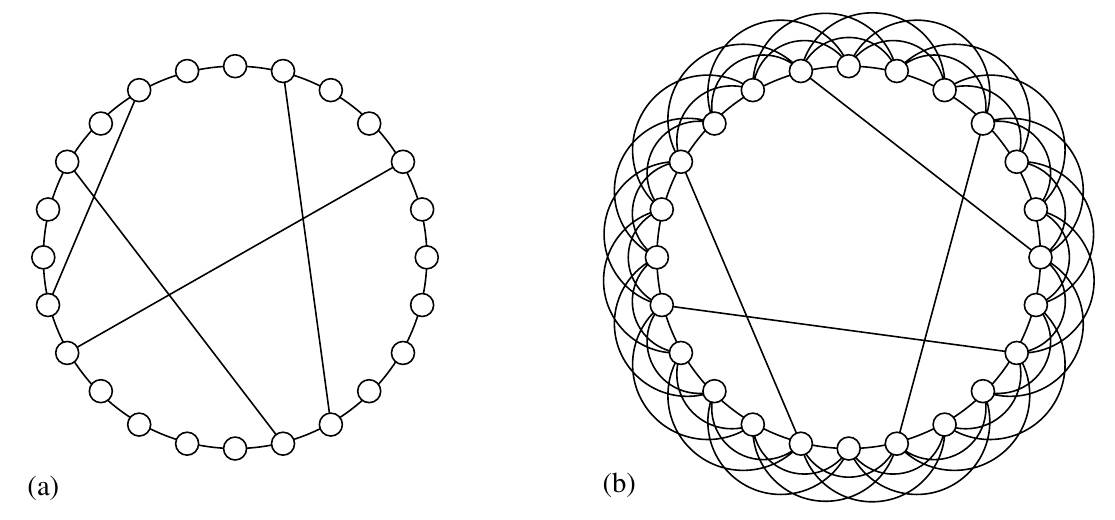
\includegraphics[width=0.9\textwidth]{figures/7olKNVY.png}
    \caption{Small-world networks with an underlying ring structure. (a) A small-world network formed by adding shortcuts to a simple ring (with $k = 1$). (b) A small-world network formed by adding shortcuts to a ring with $k = 3$.}
    \label{fig:fig1}
\end{figure}

\subsection{Clustering in a small-world network}

\nd The simplest way to treat clustering analytically in a small-world network is to use the link addition, rather than the rewiring model. In the limit of large network size, $N \to \infty$, and for a fixed fraction of shortcuts $\phi$, it is clear that the probability of forming triangle vanishes as we approach $1/N$, so the contribution of the shortcuts to the clustering is negligible. Therefore, the clustering of a small-world network is determined by its underlying ordered lattice. For example, consider a ring where each node is connected to its $k$ closest neighbors from each side. A node's number of neighbors is therefore $2k$, and thus it has $2k(2k - 1)/2 = k(2k - 1)$ pairs of neighbors. Consider a node, $i$. All of the $k$ nearest nodes on $i$'s left are connected to each other, and the same is true for the nodes on $i$'s right. This amounts to $2k(k - 1)/2 = k(k - 1)$ pairs. Now consider a node located $d$ places to the left of $k$. It is also connected to its $k$ nearest neighbors from each side. Therefore, it will be connected to $k - d$ neighbors on $i$'s right side. The total number of connected neighbor pairs is

\begin{equation}
    k(k-1) + \sum_{d=1}^k (k-d) = k(k-1) + \frac{k(k-1)}{2} = \frac{{3}{2}} k (k-1)
\end{equation}

\nd and the clustering coefficient is:

\begin{equation}
    C = \frac{\frac{3}{2}k(k-1)}{k(2k-1)} =\frac{3 (k-1)}{2(2k-1)}
\end{equation}

\nd For every $k > 1$, this results in a constant larger than $0$, indicating that the clustering of a small-world network does not vanish for large networks. For large values of $k$, the clustering coefficient approaches $3/4$, that is, the clustering is very high. Note that for a regular two-dimensional grid, the  clustering by definition is zero, since no triangles exist. However, it is clear that the grid has a neighborhood structure.

\subsection{Distances in a small-world network}

The second important property of small-world networks is their small diameter, i.e., the small distance between nodes in the network. The distance in the underlying lattice behaves as the linear length of the lattice, L. Since $N \sim L^d$  where $d$ is the lattice dimension, it follows that the distance between nodes behaves as:

\begin{equation}
    l \sim L \sim N^{1/d}
\end{equation}

\nd Therefore, the underlying lattice has a finite dimension, and the distances on it behave as a power law of the number of nodes, i.e., the distance between nodes is large. However, when adding even a small fraction of shortcuts to the network, this behavior changes dramatically. \s

\nd Let's try to deduce the behavior of the average distance between nodes. Consider a small-world network, with dimension d and connecting distance $k$ (i.e., every node is connected to any other node whose distance from it in every linear dimension is at most $k$). Now, consider the nodes reachable from a source node with at most $r$ steps. When $r$ is small, these are just the \emph{r-th} nearest neighbors of the source in the underlying lattice. We term the set of these neighbors a “patch”. the radius of which is $kr$ , and the number of nodes it contains is approximately $n(r) = (2kr)d$. \s

\nd We now want to find the distance r for which such a patch will contain about one shortcut. This will allow us to consider this patch as if it was a single node in a randomly connected network. Assume that the probability for a single node to have a shortcut is $\Phi$. To find the length for which approximately one shortcut is encountered, we need to solve for $r$ the following equation: $(2kr)^d \Phi = 1$. The correlation length $\xi$ defined as the distance (or linear size of a patch) for which a shortcut will be encountered with high probability is therefore,

\begin{equation}
    \xi = \frac{1}{k \Phi^{1/d}}
\end{equation}

\nd Note that we have omitted the factor 2, since we are interested in the order of magnitude. Let us denote by $V(r)$ the total number of nodes reachable from a node by at most $r$ steps, and by $a(r)$, the number of nodes added to a patch in the \emph{r-th} step. That is, $a(r) = n(r) - n(r-1)$. Thus,

\begin{equation}
    a(r) \sim \frac{\text{d} n(r)}{\text{d} r} = 2kd(2kr)^{d-1}
\end{equation}

\nd When a shortcut is encountered at the r step from a node, it leads to a new patch \footnote{It may actually lead to an already encountered patch, and two patches may also merge after some steps, but this occurs with negligible probability when $N \to \infty$ until most of the network is reachable}. This new patch occurs after $r'$ steps, and therefore the number of nodes reachable from its origin is $V (r - r')$. Thus, we obtain the recursive relation

\begin{equation} \label{eq:recursion}
    V(r) = \sum_{r'=0}^r a(r') [1 + \xi^{-d}V(r-r')]
\end{equation}

\nd where the first term stands for the size of the original patch, and the second term is derived from the probability of hitting a shortcut, which is approximately $\xi -d $ for every new node encountered. To simplify the solution of \ref{eq:recursion}, it can be approximated by a differential equation. The sum can be approximated by an integral, and then the equation can be differentiated with respect to $r$ . For simplicity, we will concentrate here on the solution for the one-dimensional case, with $k = 1$, where $a(r) = 2$. Thus, one obtains

\begin{equation}
    \frac{\text{d} V(r)}{\text{d} r} = 2 [1 + V(r)/\xi]
\end{equation}

\nd the solution of which is:

\begin{equation} \label{eq:V(r)}
    V(r) = \xi \left(e^{2r/\xi} -1\right)
\end{equation}

\nd For $r \ll \xi$, the exponent can be expanded in a power series, and one obtains $V(r) \sim 2r = n(r)$, as expected, since usually no shortcut is encountered. For $r \ gg \xi$, $V(r)$. An approximation for the average distance between nodes can be obtained by equating $V(r)$ from \ref*{eq:V(r)} to the total number of nodes, $V(r) = N$. This results in

\begin{equation} \label{eq:average distance}
    r \sim \frac{\xi}{2} \ln \frac{N}{\xi}
\end{equation}

\nd As apparent from \ref{eq:average distance}, the average distance in a small-world network behaves as the distance in a random graph with patches of size $\xi$ behaving as the nodes of the random graph.

\section{Detecting Small-Worldness}

As we have seen, many real technological, biological, social, and information networks fall into the broad class of \emph{small-world} networks, a middle ground between regular and random networks: they have high local clustering of elements, like regular networks, but also short path lengths between elements, like random networks. Membership of the small-world network class also implies that the corresponding systems have dynamic properties different from those of equivalent random or regular networks. \s

\nd However, the existing \emph{small-world} definition is a categorical one, and breaks the continuum of network topologies into the three classes of regular, random, and small-world networks, with the latter being the broadest. It is unclear to what extent the real-world systems in the small-world class have common network properties and to what specific point in the \emph{middle-ground} (between random and regular) a network generating model must be tuned to genuinely capture the topology of such systems. \s

\nd The current \emph{state of the art} algorithm in the field of small-world network analysis is based on the idea that small-world networks should have some topological structure, reflected by properties such as an high clustering coefficient. On the other hand, random networks (as the Erd\H{o}s-R\'enyi model) have no such structure and, usually, a low clustering coefficient. The current \emph{state of the art} algorithms can be empirically described in the following steps:

\begin{enumerate}
    \item Compute the average shortest path length $L$ and the average clustering coefficient $C$ of the target system.
    \item Create an ensemble of random networks with the same number of nodes and edges as the target system. Usually, the random networks are generated using the Erd\H{o}s-R\'enyi model.
    \item Compute the average shortest path length $L_r$ and the average clustering coefficient $C_r$ of each random network in the ensemble.
    \item Compute the normalized average shortest path length $\lambda := L/L_n$ and the normalized average clustering coefficient $\gamma := C/C_n$
    \item If $\lambda$ and $\gamma$ are close to 1, then the target system is a small-world network.
\end{enumerate}

\nd One of the problems with this interpretations is that we have no information on how the average shortest path scales with the network size. Specifically, a small-world network is defined to be a network where the typical distance $L$ between two randomly chosen nodes (the number of steps required) grows proportionally to the logarithm of the number of nodes $N$ in the network.
$$ L \propto N $$
But since we are working with a real-world network, there is no such thing as "same network with different number of nodes". So this definition, can't be applied in this case. \s

\nd Furthermore, let's try to take another approach. We can consider a definition of small-world network that it's not directly depend of $\gamma$ and $\lambda$, e.g:

\begin{center}
    \emph{A small-world network is a spatial network with added long-range connections}.
\end{center}

\nd Then we still cannot make robust implications as to whether such a definition is fulfilled just using $\gamma$ and $\lambda$ (or in fact other network measures). The interpretation of many studies assumes that all networks are a realization of the Watts-Strogatz model for some rewiring probability, which is not justified at all! We know many other network models, whose realizations are entirely different from the Watts-Strogatz model. \s

\nd The above method is not robust to measurement errors. Small errors when establishing a network from measurements suffice to make, e.g., a lattice look like a small-world network. See \cite{https://doi.org/10.48550/arxiv.1111.4570} and \cite{10.3389/fnhum.2016.00096}. \s



\clearpage
\bibliographystyle{unsrt}
\bibliography{ref}
\nocite{*}
\end{document}
